\documentclass[nofonts,]{tufte-handout}

% ams
\usepackage{amssymb,amsmath}

\usepackage{ifxetex,ifluatex}
\usepackage{fixltx2e} % provides \textsubscript
\ifnum 0\ifxetex 1\fi\ifluatex 1\fi=0 % if pdftex
  \usepackage[T1]{fontenc}
  \usepackage[utf8]{inputenc}
\else % if luatex or xelatex
  \makeatletter
  \@ifpackageloaded{fontspec}{}{\usepackage{fontspec}}
  \makeatother
  \defaultfontfeatures{Ligatures=TeX,Scale=MatchLowercase}
  \makeatletter
  \@ifpackageloaded{soul}{
     \renewcommand\allcapsspacing[1]{{\addfontfeature{LetterSpace=15}#1}}
     \renewcommand\smallcapsspacing[1]{{\addfontfeature{LetterSpace=10}#1}}
   }{}
  \makeatother
\fi

% graphix
\usepackage{graphicx}
\setkeys{Gin}{width=\linewidth,totalheight=\textheight,keepaspectratio}

% booktabs
\usepackage{booktabs}

% url
\usepackage{url}

% hyperref
\usepackage{hyperref}

% units.
\usepackage{units}


\setcounter{secnumdepth}{-1}

% citations
\usepackage{natbib}
\bibliographystyle{plainnat}

%% tint override
\setcitestyle{round} 

% pandoc syntax highlighting
\usepackage{color}
\usepackage{fancyvrb}
\newcommand{\VerbBar}{|}
\newcommand{\VERB}{\Verb[commandchars=\\\{\}]}
\DefineVerbatimEnvironment{Highlighting}{Verbatim}{commandchars=\\\{\}}
% Add ',fontsize=\small' for more characters per line
\usepackage{framed}
\definecolor{shadecolor}{RGB}{248,248,248}
\newenvironment{Shaded}{\begin{snugshade}}{\end{snugshade}}
\newcommand{\AlertTok}[1]{\textcolor[rgb]{0.94,0.16,0.16}{#1}}
\newcommand{\AnnotationTok}[1]{\textcolor[rgb]{0.56,0.35,0.01}{\textbf{\textit{#1}}}}
\newcommand{\AttributeTok}[1]{\textcolor[rgb]{0.77,0.63,0.00}{#1}}
\newcommand{\BaseNTok}[1]{\textcolor[rgb]{0.00,0.00,0.81}{#1}}
\newcommand{\BuiltInTok}[1]{#1}
\newcommand{\CharTok}[1]{\textcolor[rgb]{0.31,0.60,0.02}{#1}}
\newcommand{\CommentTok}[1]{\textcolor[rgb]{0.56,0.35,0.01}{\textit{#1}}}
\newcommand{\CommentVarTok}[1]{\textcolor[rgb]{0.56,0.35,0.01}{\textbf{\textit{#1}}}}
\newcommand{\ConstantTok}[1]{\textcolor[rgb]{0.00,0.00,0.00}{#1}}
\newcommand{\ControlFlowTok}[1]{\textcolor[rgb]{0.13,0.29,0.53}{\textbf{#1}}}
\newcommand{\DataTypeTok}[1]{\textcolor[rgb]{0.13,0.29,0.53}{#1}}
\newcommand{\DecValTok}[1]{\textcolor[rgb]{0.00,0.00,0.81}{#1}}
\newcommand{\DocumentationTok}[1]{\textcolor[rgb]{0.56,0.35,0.01}{\textbf{\textit{#1}}}}
\newcommand{\ErrorTok}[1]{\textcolor[rgb]{0.64,0.00,0.00}{\textbf{#1}}}
\newcommand{\ExtensionTok}[1]{#1}
\newcommand{\FloatTok}[1]{\textcolor[rgb]{0.00,0.00,0.81}{#1}}
\newcommand{\FunctionTok}[1]{\textcolor[rgb]{0.00,0.00,0.00}{#1}}
\newcommand{\ImportTok}[1]{#1}
\newcommand{\InformationTok}[1]{\textcolor[rgb]{0.56,0.35,0.01}{\textbf{\textit{#1}}}}
\newcommand{\KeywordTok}[1]{\textcolor[rgb]{0.13,0.29,0.53}{\textbf{#1}}}
\newcommand{\NormalTok}[1]{#1}
\newcommand{\OperatorTok}[1]{\textcolor[rgb]{0.81,0.36,0.00}{\textbf{#1}}}
\newcommand{\OtherTok}[1]{\textcolor[rgb]{0.56,0.35,0.01}{#1}}
\newcommand{\PreprocessorTok}[1]{\textcolor[rgb]{0.56,0.35,0.01}{\textit{#1}}}
\newcommand{\RegionMarkerTok}[1]{#1}
\newcommand{\SpecialCharTok}[1]{\textcolor[rgb]{0.00,0.00,0.00}{#1}}
\newcommand{\SpecialStringTok}[1]{\textcolor[rgb]{0.31,0.60,0.02}{#1}}
\newcommand{\StringTok}[1]{\textcolor[rgb]{0.31,0.60,0.02}{#1}}
\newcommand{\VariableTok}[1]{\textcolor[rgb]{0.00,0.00,0.00}{#1}}
\newcommand{\VerbatimStringTok}[1]{\textcolor[rgb]{0.31,0.60,0.02}{#1}}
\newcommand{\WarningTok}[1]{\textcolor[rgb]{0.56,0.35,0.01}{\textbf{\textit{#1}}}}

% longtable

% multiplecol
\usepackage{multicol}

% strikeout
\usepackage[normalem]{ulem}

% morefloats
\usepackage{morefloats}


% tightlist macro required by pandoc >= 1.14
\providecommand{\tightlist}{%
  \setlength{\itemsep}{0pt}\setlength{\parskip}{0pt}}

% title / author / date
\title{UCSCXenaTools: R API for UCSC Xena Hubs}
\author{Shixiang Wang}
\date{2019-06-17}

%% -- tint overrides
%% fonts, using roboto (condensed) as default
\usepackage[sfdefault,condensed]{roboto}
%% also nice: \usepackage[default]{lato}

%% colored links, setting 'borrowed' from RJournal.sty with 'Thanks, Achim!'
\RequirePackage{color}
\definecolor{link}{rgb}{0.1,0.1,0.8} %% blue with some grey
\hypersetup{
  colorlinks,%
  citecolor=link,%
  filecolor=link,%
  linkcolor=link,%
  urlcolor=link
}

%% macros
\makeatletter

%% -- tint does not use italics or allcaps in title
\renewcommand{\maketitle}{%     
  \newpage
  \global\@topnum\z@% prevent floats from being placed at the top of the page
  \begingroup
    \setlength{\parindent}{0pt}%
    \setlength{\parskip}{4pt}%
    \let\@@title\@empty
    \let\@@author\@empty
    \let\@@date\@empty
    \ifthenelse{\boolean{@tufte@sfsidenotes}}{%
      %\gdef\@@title{\sffamily\LARGE\allcaps{\@title}\par}%
      %\gdef\@@author{\sffamily\Large\allcaps{\@author}\par}%
      %\gdef\@@date{\sffamily\Large\allcaps{\@date}\par}%
      \gdef\@@title{\begingroup\fontseries{b}\selectfont\LARGE{\@title}\par}%
      \gdef\@@author{\begingroup\fontseries{l}\selectfont\Large{\@author}\par}%
      \gdef\@@date{\begingroup\fontseries{l}\selectfont\Large{\@date}\par}%
    }{%
      %\gdef\@@title{\LARGE\itshape\@title\par}%
      %\gdef\@@author{\Large\itshape\@author\par}%
      %\gdef\@@date{\Large\itshape\@date\par}%
      \gdef\@@title{\begingroup\fontseries{b}\selectfont\LARGE\@title\par\endgroup}%
      \gdef\@@author{\begingroup\fontseries{l}\selectfont\Large\@author\par\endgroup}%
      \gdef\@@date{\begingroup\fontseries{l}\selectfont\Large\@date\par\endgroup}%
    }%
    \@@title
    \@@author
    \@@date
  \endgroup
  \thispagestyle{plain}% suppress the running head
  \tuftebreak% add some space before the text begins
  \@afterindentfalse\@afterheading% suppress indentation of the next paragraph
}

%% -- tint does not use italics or allcaps in section/subsection/paragraph
\titleformat{\section}%
  [hang]% shape
  %{\normalfont\Large\itshape}% format applied to label+text
  {\fontseries{b}\selectfont\Large}% format applied to label+text
  {\thesection}% label
  {1em}% horizontal separation between label and title body
  {}% before the title body
  []% after the title body

\titleformat{\subsection}%
  [hang]% shape
  %{\normalfont\large\itshape}% format applied to label+text
  {\fontseries{m}\selectfont\large}% format applied to label+text
  {\thesubsection}% label
  {1em}% horizontal separation between label and title body
  {}% before the title body
  []% after the title body

\titleformat{\paragraph}%
  [runin]% shape
  %{\normalfont\itshape}% format applied to label+text
  {\fontseries{l}\selectfont}% format applied to label+text
  {\theparagraph}% label
  {1em}% horizontal separation between label and title body
  {}% before the title body
  []% after the title body

%% -- tint does not use italics here either
% Formatting for main TOC (printed in front matter)
% {section} [left] {above} {before w/label} {before w/o label} {filler + page} [after]
\ifthenelse{\boolean{@tufte@toc}}{%
  \titlecontents{part}% FIXME
    [0em] % distance from left margin
    %{\vspace{1.5\baselineskip}\begin{fullwidth}\LARGE\rmfamily\itshape} % above (global formatting of entry)
    {\vspace{1.5\baselineskip}\begin{fullwidth}\fontseries{m}\selectfont\LARGE} % above (global formatting of entry)
    {\contentslabel{2em}} % before w/label (label = ``II'')
    {} % before w/o label
    {\rmfamily\upshape\qquad\thecontentspage} % filler + page (leaders and page num)
    [\end{fullwidth}] % after
  \titlecontents{chapter}%
    [0em] % distance from left margin
    %{\vspace{1.5\baselineskip}\begin{fullwidth}\LARGE\rmfamily\itshape} % above (global formatting of entry)
    {\vspace{1.5\baselineskip}\begin{fullwidth}\fontseries{m}\selectfont\LARGE} % above (global formatting of entry)
    {\hspace*{0em}\contentslabel{2em}} % before w/label (label = ``2'')
    {\hspace*{0em}} % before w/o label
    %{\rmfamily\upshape\qquad\thecontentspage} % filler + page (leaders and page num)
    {\upshape\qquad\thecontentspage} % filler + page (leaders and page num)
    [\end{fullwidth}] % after
  \titlecontents{section}% FIXME
    [0em] % distance from left margin
    %{\vspace{0\baselineskip}\begin{fullwidth}\Large\rmfamily\itshape} % above (global formatting of entry)
    {\vspace{0\baselineskip}\begin{fullwidth}\fontseries{m}\selectfont\Large} % above (global formatting of entry)
    {\hspace*{2em}\contentslabel{2em}} % before w/label (label = ``2.6'')
    {\hspace*{2em}} % before w/o label
    %{\rmfamily\upshape\qquad\thecontentspage} % filler + page (leaders and page num)
    {\upshape\qquad\thecontentspage} % filler + page (leaders and page num)
    [\end{fullwidth}] % after
  \titlecontents{subsection}% FIXME
    [0em] % distance from left margin
    %{\vspace{0\baselineskip}\begin{fullwidth}\large\rmfamily\itshape} % above (global formatting of entry)
    {\vspace{0\baselineskip}\begin{fullwidth}\fontseries{m}\selectfont\large} % above (global formatting of entry)
    {\hspace*{4em}\contentslabel{4em}} % before w/label (label = ``2.6.1'')
    {\hspace*{4em}} % before w/o label
    %{\rmfamily\upshape\qquad\thecontentspage} % filler + page (leaders and page num)
    {\upshape\qquad\thecontentspage} % filler + page (leaders and page num)
    [\end{fullwidth}] % after
  \titlecontents{paragraph}% FIXME
    [0em] % distance from left margin
    %{\vspace{0\baselineskip}\begin{fullwidth}\normalsize\rmfamily\itshape} % above (global formatting of entry)
    {\vspace{0\baselineskip}\begin{fullwidth}\fontseries{m}\selectfont\normalsize\rmfamily} % above (global formatting of entry)
    {\hspace*{6em}\contentslabel{2em}} % before w/label (label = ``2.6.0.0.1'')
    {\hspace*{6em}} % before w/o label
    %{\rmfamily\upshape\qquad\thecontentspage} % filler + page (leaders and page num)
    {\upshape\qquad\thecontentspage} % filler + page (leaders and page num)
    [\end{fullwidth}] % after
}{}

  
\makeatother



\begin{document}

\maketitle




This vignette gives users the summary information of API functions
provided by \textbf{UCSCXenaTools} for UCSC Xena.

Before using API, user should know some concepts about Xena elements.
Following description is copied from
\href{https://github.com/ucscXena/xenaPython/blob/master/xenaPython/__init__.py}{xenaPython
\texttt{\_\_init\_\_.py}}.

\begin{quote}
Data rows are associated with ``sample'' IDs.

Sample IDs are unique within a ``\textbf{cohort}''. s A
``\textbf{dataset}'' is a particular assay of a cohort, e.g.~gene
expression.

Datasets have associated metadata, specifying their data type and
cohort.

There are three primary data types: \textbf{dense matrix} (samples by
probes), \textbf{sparse} (sample, position, variant), and
\textbf{segmented} (sample, position, value).

Dense matrices can be genotypic or phenotypic. Phenotypic matrices have
associated \textbf{field metadata} (descriptive names, codes, etc.).
Genotypic matricies may have an associated \textbf{probeMap}, which maps
probes to genomic locations. If a matrix has hugo probeMap, the probes
themselves are gene names. Otherwise, a probeMap is used to map a gene
location to a set of probes.
\end{quote}

\hypertarget{new-features}{%
\section{New features}\label{new-features}}

A new series of functions (mostly) starting with \texttt{fetch\_} have
been introduced to help fetch a small amount of data by Xena APIs.

Now three are available:

\begin{itemize}
\tightlist
\item
  \texttt{fetch\_dense\_values()}: fetches values from a dense matrix.
\item
  \texttt{fetch\_dataset\_samples()}: fetches samples from a dataset
\item
  \texttt{fetch\_dataset\_identifiers()}: fetches identifies from a
  dataset.
\end{itemize}

They have similar arguments and all the details can be viewed by running
\texttt{?fetch} in R console after \texttt{library(UCSCXenaTools)}.

\hypertarget{api-categories}{%
\section{API categories}\label{api-categories}}

API functions can be divided into two classes: \textbf{lower API
functions} and \textbf{higher API functions}. They have following
difference:

\begin{itemize}
\tightlist
\item
  The main difference between them is that the target of higher API
  functions is \texttt{XenaHub} object, which is a S4 class built in R.
  While the targets of lower API functions are Xena hub urls, cohort
  names or dataset names with character format. The \texttt{XenaHub}
  object can provide more uniform operation methods and can be used to
  download corresponding datasets quickly and easily (detail see
  \href{https://shixiangwang.github.io/home/en/tools/ucscxenatools-intro/}{another
  vignette}).
\item
  Lower API functions are not registered in package
  \href{https://github.com/ShixiangWang/UCSCXenaTools/blob/master/NAMESPACE}{NAMESPACE},
  so user may not access them after \texttt{library(UCSCXenaTools)},
  user need to use \texttt{UCSCXenaTools:::fun\_name} instead.
\item
  Lower API functions have no help pages, so user cannot find any
  description about them in R, which means you cannot use
  \texttt{?fun\_name} to get help. However, API report part in this
  vignette shows all avaiable API functions and their short description.
\item
  Higher API functions are built on lower API functions, they return
  more meaningful and easy results for operation. Most of lower API
  functions return nested lists as results, user need to tidy them
  before using them in next step.
\end{itemize}

\hypertarget{lower-api-functions}{%
\subsection{Lower API functions}\label{lower-api-functions}}

Lower API functions also have 2 classes:

\begin{itemize}
\item
  one is generated from
  \href{https://github.com/ShixiangWang/UCSCXenaTools/tree/master/inst/queries}{\texttt{.xq}
  files}, function names all start with \texttt{.p\_}. All \texttt{.xq}
  files are copied from
  \href{https://github.com/ucscXena/xenaPython}{xenaPython} package,
  which is official Python API for Xena. These functions are dynamicly
  created when \textbf{UCSCXenaTools} loaded. Their names are given as
  following:

\begin{verbatim}
#>  [1] ".p_all_cohorts"                    
#>  [2] ".p_all_datasets"                   
#>  [3] ".p_all_datasets_n"                 
#>  [4] ".p_all_field_metadata"             
#>  [5] ".p_cohort_samples"                 
#>  [6] ".p_cohort_summary"                 
#>  [7] ".p_dataset_fetch"                  
#>  [8] ".p_dataset_field"                  
#>  [9] ".p_dataset_field_examples"         
#> [10] ".p_dataset_field_n"                
#> [11] ".p_dataset_gene_probe_avg"         
#> [12] ".p_dataset_gene_probes_values"     
#> [13] ".p_dataset_list"                   
#> [14] ".p_dataset_metadata"               
#> [15] ".p_dataset_probe_signature"        
#> [16] ".p_dataset_probe_values"           
#> [17] ".p_dataset_samples"                
#> [18] ".p_dataset_samples_ndense_matrix"  
#> [19] ".p_datasets_null_rows"             
#> [20] ".p_feature_list"                   
#> [21] ".p_field_codes"                    
#> [22] ".p_field_metadata"                 
#> [23] ".p_gene_transcripts"               
#> [24] ".p_match_fields"                   
#> [25] ".p_probe_count"                    
#> [26] ".p_probemap_list"                  
#> [27] ".p_ref_gene_exons"                 
#> [28] ".p_ref_gene_position"              
#> [29] ".p_ref_gene_range"                 
#> [30] ".p_segment_data_examples"          
#> [31] ".p_segmented_data_range"           
#> [32] ".p_sparse_data"                    
#> [33] ".p_sparse_data_examples"           
#> [34] ".p_sparse_data_match_field"        
#> [35] ".p_sparse_data_match_field_slow"   
#> [36] ".p_sparse_data_match_partial_field"
#> [37] ".p_sparse_data_range"              
#> [38] ".p_transcript_expression"
\end{verbatim}
\item
  the other one is created in package. The function names all start with
  \texttt{.}, are given as following:

\begin{verbatim}
#> [1] ".host_cohorts"         
#> [2] ".cohort_datasets"      
#> [3] ".cohort_datasets_count"
#> [4] ".cohort_samples_each"  
#> [5] ".cohort_samples_any"   
#> [6] ".cohort_samples_all"   
#> [7] ".dataset_samples_each" 
#> [8] ".dataset_samples_any"  
#> [9] ".dataset_samples_all"
\end{verbatim}
\end{itemize}

I don't know how to write these query sentence for Xena Hubs. So here I
want to say thanks to authors of
\href{https://github.com/ucscXena/xenaPython}{\textbf{xenaPython}} and
\href{https://github.com/mtmorgan/XenaR}{\textbf{xenaR}} packages.

\hypertarget{api-report}{%
\section{API report}\label{api-report}}

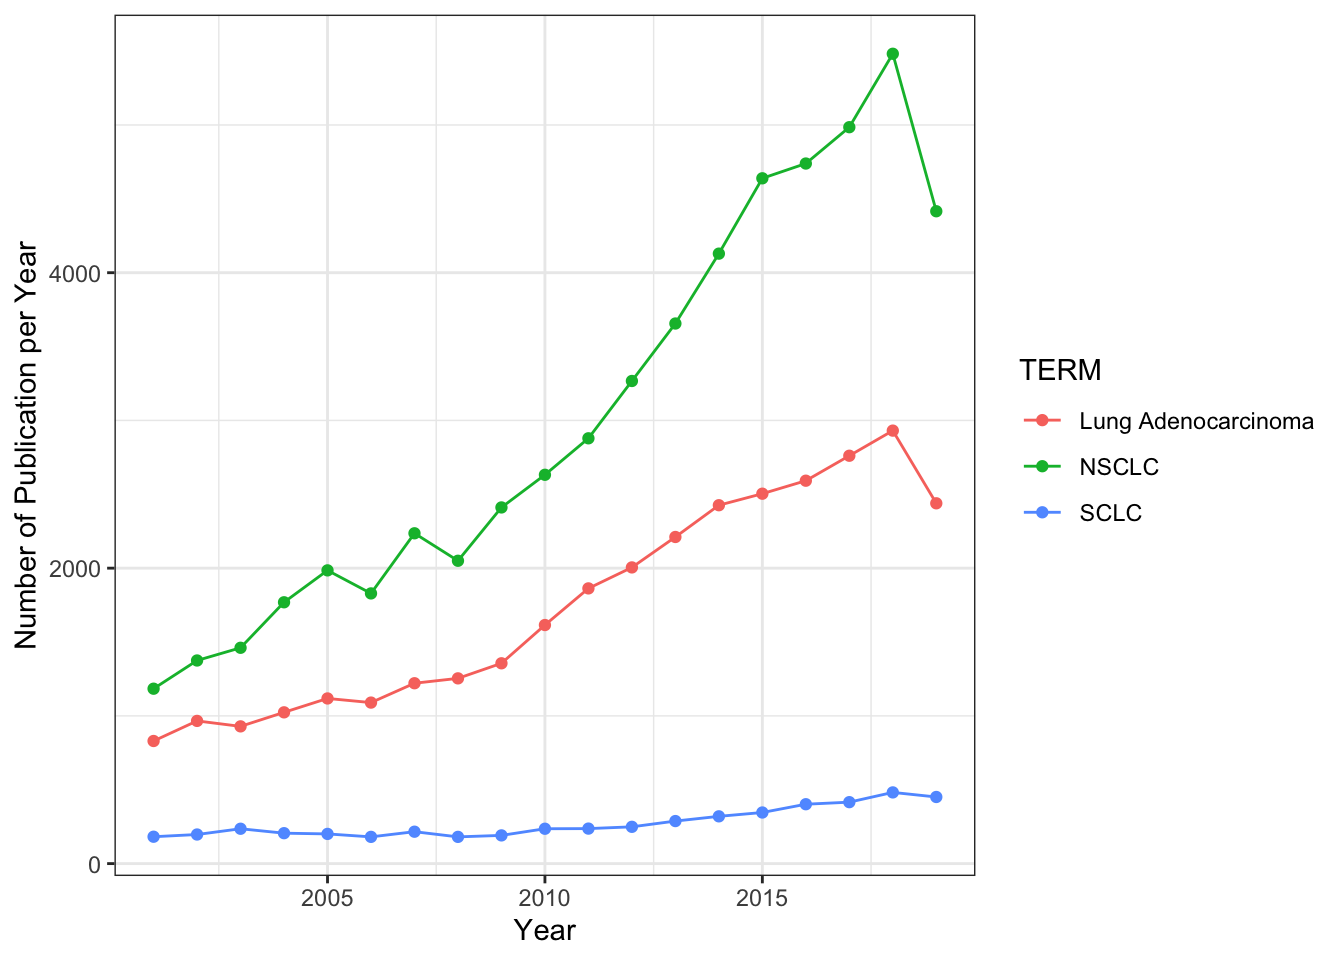
\includegraphics{ucscxenatools-api_files/figure-latex/unnamed-chunk-4-1}

Of note, I don't know test all functions generated from \texttt{.xq}
files, most of them works. Sometimes functions return you errors or
\texttt{list()} may caused by invaild format or bad network, you should
try more times. If you make sure there are problems/errors in query
procedure, you can check corresponding query variables:

\begin{verbatim}
#>  [1] ".xq_all_cohorts"                    
#>  [2] ".xq_all_datasets"                   
#>  [3] ".xq_all_datasets_n"                 
#>  [4] ".xq_all_field_metadata"             
#>  [5] ".xq_cohort_samples"                 
#>  [6] ".xq_cohort_summary"                 
#>  [7] ".xq_dataset_fetch"                  
#>  [8] ".xq_dataset_field"                  
#>  [9] ".xq_dataset_field_examples"         
#> [10] ".xq_dataset_field_n"                
#> [11] ".xq_dataset_gene_probe_avg"         
#> [12] ".xq_dataset_gene_probes_values"     
#> [13] ".xq_dataset_list"                   
#> [14] ".xq_dataset_metadata"               
#> [15] ".xq_dataset_probe_signature"        
#> [16] ".xq_dataset_probe_values"           
#> [17] ".xq_dataset_samples"                
#> [18] ".xq_dataset_samples_ndense_matrix"  
#> [19] ".xq_datasets_null_rows"             
#> [20] ".xq_feature_list"                   
#> [21] ".xq_field_codes"                    
#> [22] ".xq_field_metadata"                 
#> [23] ".xq_gene_transcripts"               
#> [24] ".xq_match_fields"                   
#> [25] ".xq_probe_count"                    
#> [26] ".xq_probemap_list"                  
#> [27] ".xq_ref_gene_exons"                 
#> [28] ".xq_ref_gene_position"              
#> [29] ".xq_ref_gene_range"                 
#> [30] ".xq_segment_data_examples"          
#> [31] ".xq_segmented_data_range"           
#> [32] ".xq_sparse_data"                    
#> [33] ".xq_sparse_data_examples"           
#> [34] ".xq_sparse_data_match_field"        
#> [35] ".xq_sparse_data_match_field_slow"   
#> [36] ".xq_sparse_data_match_partial_field"
#> [37] ".xq_sparse_data_range"              
#> [38] ".xq_transcript_expression"
\end{verbatim}

For example, you'd like to check \texttt{.p\_all\_cohorts} function, you
can take a look at \texttt{.xq\_all\_cohorts} object.

\begin{Shaded}
\begin{Highlighting}[]
\NormalTok{.xq_all_cohorts}
\CommentTok{#> [1] ";allCohorts\textbackslash{}n(fn [exclude]\textbackslash{}n\textbackslash{}t(map :cohort\textbackslash{}n\textbackslash{}t  (query\textbackslash{}n\textbackslash{}t\textbackslash{}t\{:select [[#sql/call [:distinct #sql/call [:ifnull :cohort \textbackslash{}"(unassigned)\textbackslash{}"]] :cohort]]\textbackslash{}n\textbackslash{}t\textbackslash{}t :from [:dataset]\textbackslash{}n\textbackslash{}t\textbackslash{}t :where [:not [:in :type exclude]]\})))\textbackslash{}n"}
\end{Highlighting}
\end{Shaded}

\texttt{cat} it may give you more easy-to-read format.

\begin{Shaded}
\begin{Highlighting}[]
\KeywordTok{cat}\NormalTok{(.xq_all_cohorts)}
\CommentTok{#> ;allCohorts}
\CommentTok{#> (fn [exclude]}
\CommentTok{#>  (map :cohort}
\CommentTok{#>    (query}
\CommentTok{#>      \{:select [[#sql/call [:distinct #sql/call [:ifnull :cohort "(unassigned)"]] :cohort]]}
\CommentTok{#>       :from [:dataset]}
\CommentTok{#>       :where [:not [:in :type exclude]]\})))}
\end{Highlighting}
\end{Shaded}

\hypertarget{use-cases}{%
\section{Use cases}\label{use-cases}}

Several use cases are modified from
\href{https://github.com/ucscXena/xenaPython}{README} of
\textbf{xenaPython} package.

Load package firstly.

\begin{Shaded}
\begin{Highlighting}[]
\KeywordTok{library}\NormalTok{(UCSCXenaTools)}
\end{Highlighting}
\end{Shaded}

You can find out host id and dataset id from
\url{https://xenabrowser.net/datapages/}, a more recommened way is use
\texttt{XenaData} in \textbf{UCSCXenaTools}.

\begin{Shaded}
\begin{Highlighting}[]
\KeywordTok{head}\NormalTok{(XenaData)[, }\DecValTok{1}\OperatorTok{:}\DecValTok{5}\NormalTok{]}
\CommentTok{#> # A tibble: 6 x 5}
\CommentTok{#>   XenaHosts XenaHostNames XenaCohorts}
\CommentTok{#>   <chr>     <chr>         <chr>      }
\CommentTok{#> 1 https://~ publicHub     Acute lymp~}
\CommentTok{#> 2 https://~ publicHub     Acute lymp~}
\CommentTok{#> 3 https://~ publicHub     Acute lymp~}
\CommentTok{#> 4 https://~ publicHub     Breast Can~}
\CommentTok{#> 5 https://~ publicHub     Breast Can~}
\CommentTok{#> 6 https://~ publicHub     Breast Can~}
\CommentTok{#> # ... with 2 more variables:}
\CommentTok{#> #   XenaDatasets <chr>, SampleCount <chr>}
\end{Highlighting}
\end{Shaded}

The host id is stored at \texttt{XenaHosts} column, and dataset id is
stored at \texttt{XenaDatasets} column.

\textbf{Of note, when you want to query single sample or gene with
function starts with \texttt{.p\_}, you must transform id of sample or
gene into a \texttt{list}}

\hypertarget{query-four-samples-and-three-identifers-expression}{%
\subsection{Query four samples and three identifers
expression}\label{query-four-samples-and-three-identifers-expression}}

\begin{Shaded}
\begin{Highlighting}[]
\NormalTok{hub =}\StringTok{ "https://toil.xenahubs.net"}
\NormalTok{dataset =}\StringTok{ "tcga_RSEM_gene_tpm"}
\NormalTok{samples =}\StringTok{ }\KeywordTok{c}\NormalTok{(}\StringTok{"TCGA-02-0047-01"}\NormalTok{, }\StringTok{"TCGA-02-0055-01"}\NormalTok{, }
    \StringTok{"TCGA-02-2483-01"}\NormalTok{, }\StringTok{"TCGA-02-2485-01"}\NormalTok{)}
\NormalTok{probes =}\StringTok{ }\KeywordTok{c}\NormalTok{(}\StringTok{"ENSG00000282740.1"}\NormalTok{, }\StringTok{"ENSG00000000005.5"}\NormalTok{, }
    \StringTok{"ENSG00000000419.12"}\NormalTok{)}
\KeywordTok{.p_dataset_probe_values}\NormalTok{(hub, dataset, samples, }
\NormalTok{    probes)}
\CommentTok{#> [[1]]}
\CommentTok{#>   strand  chromend chromstart chrom}
\CommentTok{#> 1      -  16750589   16739938  chr1}
\CommentTok{#> 2      -  50958555   50934867 chr20}
\CommentTok{#> 3      + 100599885  100584802  chrX}
\CommentTok{#> }
\CommentTok{#> [[2]]}
\CommentTok{#>        [,1]   [,2]   [,3]   [,4]}
\CommentTok{#> [1,] -9.966 -2.826 -9.966 -9.966}
\CommentTok{#> [2,] -3.171  4.165 -5.574 -3.171}
\CommentTok{#> [3,]  4.675  6.025  5.826  5.177}
\end{Highlighting}
\end{Shaded}

Query one probe. As metioned above, one must transform id of proble or
sample int a \texttt{list} when he wants to query only one sample/probe.

\textbf{Bad query}:

\begin{Shaded}
\begin{Highlighting}[]
\KeywordTok{.p_dataset_probe_values}\NormalTok{(hub, dataset, samples, }
    \StringTok{"ENSG00000282740.1"}\NormalTok{)}
\CommentTok{#> [[1]]}
\CommentTok{#> list()}
\CommentTok{#> }
\CommentTok{#> [[2]]}
\CommentTok{#>       [,1] [,2] [,3] [,4]}
\CommentTok{#>  [1,]  NaN  NaN  NaN  NaN}
\CommentTok{#>  [2,]  NaN  NaN  NaN  NaN}
\CommentTok{#>  [3,]  NaN  NaN  NaN  NaN}
\CommentTok{#>  [4,]  NaN  NaN  NaN  NaN}
\CommentTok{#>  [5,]  NaN  NaN  NaN  NaN}
\CommentTok{#>  [6,]  NaN  NaN  NaN  NaN}
\CommentTok{#>  [7,]  NaN  NaN  NaN  NaN}
\CommentTok{#>  [8,]  NaN  NaN  NaN  NaN}
\CommentTok{#>  [9,]  NaN  NaN  NaN  NaN}
\CommentTok{#> [10,]  NaN  NaN  NaN  NaN}
\CommentTok{#> [11,]  NaN  NaN  NaN  NaN}
\CommentTok{#> [12,]  NaN  NaN  NaN  NaN}
\CommentTok{#> [13,]  NaN  NaN  NaN  NaN}
\CommentTok{#> [14,]  NaN  NaN  NaN  NaN}
\CommentTok{#> [15,]  NaN  NaN  NaN  NaN}
\CommentTok{#> [16,]  NaN  NaN  NaN  NaN}
\CommentTok{#> [17,]  NaN  NaN  NaN  NaN}
\end{Highlighting}
\end{Shaded}

\textbf{Good query}:

\begin{Shaded}
\begin{Highlighting}[]
\KeywordTok{.p_dataset_probe_values}\NormalTok{(hub, dataset, samples, }
    \KeywordTok{as.list}\NormalTok{(}\StringTok{"ENSG00000282740.1"}\NormalTok{))}
\CommentTok{#> [[1]]}
\CommentTok{#>   strand chromend chromstart chrom}
\CommentTok{#> 1      - 16750589   16739938  chr1}
\CommentTok{#> }
\CommentTok{#> [[2]]}
\CommentTok{#>        [,1]   [,2]   [,3]   [,4]}
\CommentTok{#> [1,] -9.966 -2.826 -9.966 -9.966}
\end{Highlighting}
\end{Shaded}

\hypertarget{query-four-samples-and-three-genes-expression-when-the-dataset-you-want-to-query-has-a-identifier-to-gene-mapping}{%
\subsection{Query four samples and three genes expression, when the
dataset you want to query has a identifier-to-gene
mapping}\label{query-four-samples-and-three-genes-expression-when-the-dataset-you-want-to-query-has-a-identifier-to-gene-mapping}}

\begin{quote}
identifier-to-gene mapping (i.e.~xena probeMap)
\end{quote}

\begin{Shaded}
\begin{Highlighting}[]
\NormalTok{genes =}\StringTok{ }\KeywordTok{c}\NormalTok{(}\StringTok{"TP53"}\NormalTok{, }\StringTok{"RB1"}\NormalTok{, }\StringTok{"PIK3CA"}\NormalTok{)}
\KeywordTok{.p_dataset_gene_probe_avg}\NormalTok{(hub, dataset, samples, }
\NormalTok{    genes)}
\CommentTok{#>     gene                      position}
\CommentTok{#> 1   TP53    -, 7687550, 7661779, chr17}
\CommentTok{#> 2    RB1  +, 48481986, 48303751, chr13}
\CommentTok{#> 3 PIK3CA +, 179240093, 179148114, chr3}
\CommentTok{#>                       scores}
\CommentTok{#> 1 5.799, 4.428, 6.515, 6.309}
\CommentTok{#> 2 5.867, 4.700, 4.810, 4.920}
\CommentTok{#> 3 3.547, 3.377, 2.789, 2.951}
\end{Highlighting}
\end{Shaded}

\hypertarget{if-the-dataset-does-not-have-id-to-gene-mapping-but-the-dataset-used-gene-names-as-its-identifier}{%
\subsection{If the dataset does not have id-to-gene mapping, but the
dataset used gene names as its
identifier}\label{if-the-dataset-does-not-have-id-to-gene-mapping-but-the-dataset-used-gene-names-as-its-identifier}}

In this situation, you can query gene expression like two ways above
will not work.

\begin{Shaded}
\begin{Highlighting}[]
\NormalTok{hub =}\StringTok{ "https://toil.xenahubs.net"}
\NormalTok{dataset =}\StringTok{ "tcga_RSEM_Hugo_norm_count"}
\NormalTok{samples =}\StringTok{ }\KeywordTok{c}\NormalTok{(}\StringTok{"TCGA-02-0047-01"}\NormalTok{, }\StringTok{"TCGA-02-0055-01"}\NormalTok{, }
    \StringTok{"TCGA-02-2483-01"}\NormalTok{, }\StringTok{"TCGA-02-2485-01"}\NormalTok{)}
\NormalTok{probes =}\StringTok{ }\KeywordTok{c}\NormalTok{(}\StringTok{"TP53"}\NormalTok{, }\StringTok{"RB1"}\NormalTok{, }\StringTok{"PIK3CA"}\NormalTok{)}

\KeywordTok{.p_dataset_probe_values}\NormalTok{(hub, dataset, samples, }
\NormalTok{    probes)}
\CommentTok{#> [[1]]}
\CommentTok{#>   strand  chromend chromstart chrom}
\CommentTok{#> 1      +  48481986   48303751 chr13}
\CommentTok{#> 2      -   7687550    7661779 chr17}
\CommentTok{#> 3      + 179240093  179148114  chr3}
\CommentTok{#> }
\CommentTok{#> [[2]]}
\CommentTok{#>       [,1]  [,2]  [,3]  [,4]}
\CommentTok{#> [1,] 11.63 10.68 12.65 12.15}
\CommentTok{#> [2,] 12.04 10.93 11.59 11.41}
\CommentTok{#> [3,] 10.67 10.90 10.71 10.12}
\end{Highlighting}
\end{Shaded}

\hypertarget{find-out-the-samples-in-a-dataset}{%
\subsection{Find out the samples in a
dataset}\label{find-out-the-samples-in-a-dataset}}

\begin{Shaded}
\begin{Highlighting}[]
\NormalTok{hub =}\StringTok{ "https://tcga.xenahubs.net"}
\NormalTok{dataset =}\StringTok{ "TCGA.BLCA.sampleMap/HiSeqV2"}
\KeywordTok{.p_dataset_samples}\NormalTok{(hub, dataset, }\DecValTok{10}\NormalTok{)}
\CommentTok{#>  [1] "TCGA-BT-A20R-11" "TCGA-DK-AA6S-01"}
\CommentTok{#>  [3] "TCGA-DK-A6B2-01" "TCGA-GU-A763-01"}
\CommentTok{#>  [5] "TCGA-XF-A9T4-01" "TCGA-FD-A5C1-01"}
\CommentTok{#>  [7] "TCGA-GU-A42Q-01" "TCGA-DK-A3IL-01"}
\CommentTok{#>  [9] "TCGA-XF-AAMH-01" "TCGA-FT-A61P-01"}
\CommentTok{# obtain all samples}
\KeywordTok{.p_dataset_samples}\NormalTok{(hub, dataset, }\OtherTok{NULL}\NormalTok{) }\OperatorTok\StringTok{ }\KeywordTok{head}\NormalTok{()}
\CommentTok{#> [1] "TCGA-BT-A20R-11" "TCGA-DK-AA6S-01"}
\CommentTok{#> [3] "TCGA-DK-A6B2-01" "TCGA-GU-A763-01"}
\CommentTok{#> [5] "TCGA-XF-A9T4-01" "TCGA-FD-A5C1-01"}
\end{Highlighting}
\end{Shaded}

Higher API function \texttt{samples()} has more features. It can be used
to do set operation for samples in a host.

\begin{Shaded}
\begin{Highlighting}[]
\NormalTok{xe =}\StringTok{ }\KeywordTok{XenaHub}\NormalTok{(}\DataTypeTok{cohorts =} \StringTok{"Cancer Cell Line Encyclopedia (CCLE)"}\NormalTok{)}
\CommentTok{# samples in each dataset, first host}
\NormalTok{x =}\StringTok{ }\KeywordTok{samples}\NormalTok{(xe, }\DataTypeTok{by =} \StringTok{"datasets"}\NormalTok{, }\DataTypeTok{how =} \StringTok{"each"}\NormalTok{)[[}\DecValTok{1}\NormalTok{]]}
\KeywordTok{lengths}\NormalTok{(x)  }\CommentTok{# data sets in ccle cohort on first (only) host}
\end{Highlighting}
\end{Shaded}

\hypertarget{find-out-the-identifiers-in-a-dataset}{%
\subsection{Find out the identifiers in a
dataset}\label{find-out-the-identifiers-in-a-dataset}}

\begin{Shaded}
\begin{Highlighting}[]
\NormalTok{hub =}\StringTok{ "https://tcga.xenahubs.net"}
\NormalTok{dataset =}\StringTok{ "TCGA.BLCA.sampleMap/HiSeqV2"}
\KeywordTok{.p_dataset_field}\NormalTok{(hub, dataset) }\OperatorTok\StringTok{ }\KeywordTok{head}\NormalTok{()}
\CommentTok{#> [1] "?|100130426" "?|100133144" "?|100134869"}
\CommentTok{#> [4] "?|10357"     "?|10431"     "?|136542"}
\end{Highlighting}
\end{Shaded}

\hypertarget{find-out-the-number-of-idnetifiers-in-a-dataset}{%
\subsection{Find out the number of idnetifiers in a
dataset}\label{find-out-the-number-of-idnetifiers-in-a-dataset}}

\begin{Shaded}
\begin{Highlighting}[]
\NormalTok{hub =}\StringTok{ "https://tcga.xenahubs.net"}
\NormalTok{dataset =}\StringTok{ "TCGA.BLCA.sampleMap/HiSeqV2"}
\KeywordTok{.p_dataset_field_n}\NormalTok{(hub, dataset)}
\CommentTok{#> [1] 20531}
\end{Highlighting}
\end{Shaded}

\hypertarget{license}{%
\section{LICENSE}\label{license}}

GPL-3

Please note, code from \textbf{XenaR} package under Apache 2.0 license.



\end{document}
